\documentclass{article}
%%%%%%% PACKAGES %%%%%%%%
\usepackage[utf8]{inputenc}
\usepackage{graphicx}
\usepackage{geometry}
\geometry{a4paper, margin=1in}
\usepackage{hyperref}
\usepackage{titling}
\usepackage{caption}
\usepackage{subcaption}
\usepackage{float}
\hypersetup{
    colorlinks=true,
    linkcolor=blue,
    filecolor=magenta,      
    urlcolor=cyan,
}

\title{Assignment 3\\CS 451: Computational Intelligence}
\author{Ali Asghar Yousuf $\mid$ Muhammad Murtaza}
\date{\today}

\begin{document}

\maketitle

\section{Reinforcement Learning Agent}

\subsection{Problem Statement}
The Gridworld problem is a classic reinforcement learning problem where an agent operates in a two-dimensional grid-like environment, and its goal is to navigate to a goal state while avoiding obstacles and maximizing rewards. The agent has a set of actions available at each grid cell, which can move it to a neighboring cell. The environment is stochastic, meaning that the agent's actions may not always have the intended effect, and the agent receives a reward or penalty depending on the action taken and the resulting state. The problem statement for Gridworld in reinforcement learning would be to find an optimal policy for the agent to navigate the environment, maximize rewards, and reach the goal state while minimizing the number of steps taken and avoiding obstacles.

\subsection{Solution Approach}
We have make use of Reinforcement Learning to optimize this problem making use of reward based learning. We will learn the value function using via episodic learning. The actions will be selected by the Boltzmann distribution.

\subsubsection{Initialization of the Grid}
The first step is to initialize a grid of size n x n where n is an integer. Red terminals (obstacles) are placed around the grid and Green Terminals (rewards) are placed around the grid. $\gamma$ and $\alpha$ are initially set to 0.8. You can change it to test for different runs.

\subsubsection{Agent Position}
Agent Position is selected in the grid randomly wherever there is any empty grid cell. In each episode, the agent starts with a new position.

\subsubsection{Temporal Difference Learning}
In our algorithm, we made use of TD to update the q values in each iteration. In TD learning, the agent learns directly from its experience in the environment by updating the value estimates of each state-action pair after each time step. This allows the agent to learn online and adapt to changes in the environment in real-time.
\\
By using the TD equation to update the value estimates of the previous state, the agent can learn the optimal policy through trial and error. Over time, the agent learns to associate certain states and actions with higher rewards, and it uses this knowledge to make decisions that maximize the total reward over time.
\\~\\
\textbf{Following equation was used to update the values: }
\\~\\
$V(S_{t})$ = $V(S_{t})$ + $\alpha(R_{t+1} + \gamma (V(S_{t}+1))-V(S_{t}))$

\\~\\
When the agent moves from one state to another, the value for that cell is updated using the equation above. 

\subsubsection{Boltzmann Distribution}

\begin{equation}
P(a|s) = \frac{e^{Q(s,a)/k}}{\sum_{b} e^{Q(s,b)/k}}
\end{equation}
In the Gridworld Reinforcement Learning problem, the Boltzmann distribution plays a crucial role in selecting actions for the agent. The Boltzmann distribution is a probabilistic policy that selects actions based on their estimated values and a temperature parameter. The temperature parameter controls the degree of exploration versus exploitation, where a higher temperature results in more exploration and a lower temperature results in more exploitation.
\\~\\
The Boltzmann distribution provides a way to balance exploration and exploitation during the learning process. Initially, the agent explores the environment by randomly selecting actions, and the temperature parameter is set high to encourage exploration. As the agent learns more about the environment, the temperature parameter is gradually reduced to favor exploitation of the learned information.

\subsection{Results}

\textbf{For the following parameters we observed the following results:}
\begin{itemize}
    \item Grid Size = 10 x 10
    \item Episodes = 100
    \item $\alpha$ = 0.8 
    \item $\gamma$ = 0.8
\end{itemize}

\begin{figure}[H]
  \centering
  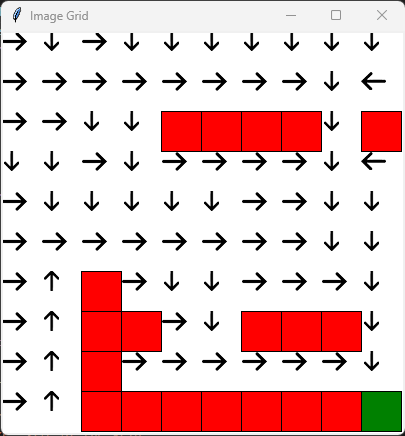
\includegraphics[width=0.4\textwidth, height=0.25\textheight]{grid_1.png}
  \caption{First Run}
\end{figure}
\\~\\
\newpage
\begin{itemize}
    \item Grid Size = 25 x 25
    \item Episodes = 500
    \item $\alpha$ = 0.8 
    \item $\gamma$ = 0.8
\end{itemize}

\begin{figure}[H]
  \centering
  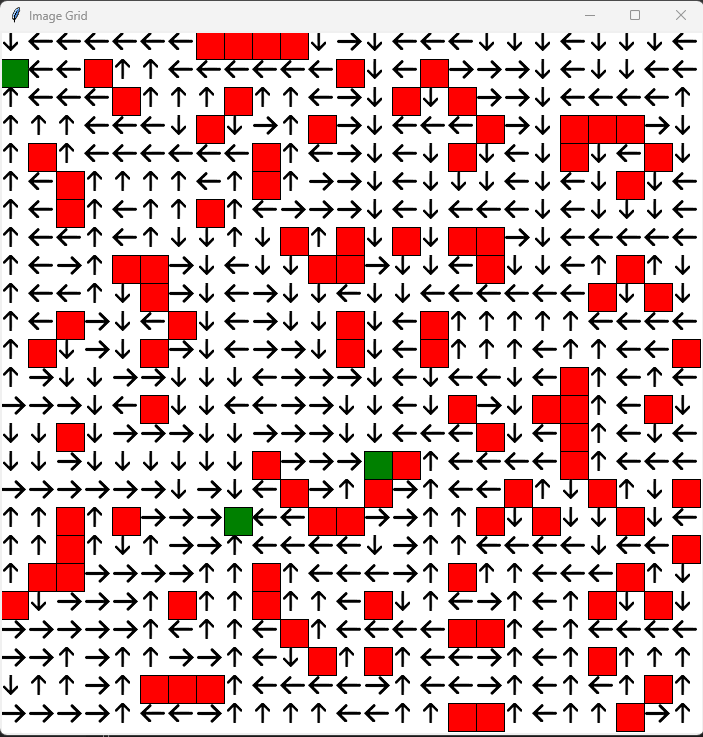
\includegraphics[width=0.5\textwidth, height=0.3\textheight]{grid_2.png}
  \caption{Second Run}
\end{figure}

\\~\\
\begin{itemize}
    \item Grid Size = 15 x 15
    \item Episodes = 250
    \item $\alpha$ = 0.2 
    \item $\gamma$ = 0.6
\end{itemize}

\begin{figure}[H]
  \centering
  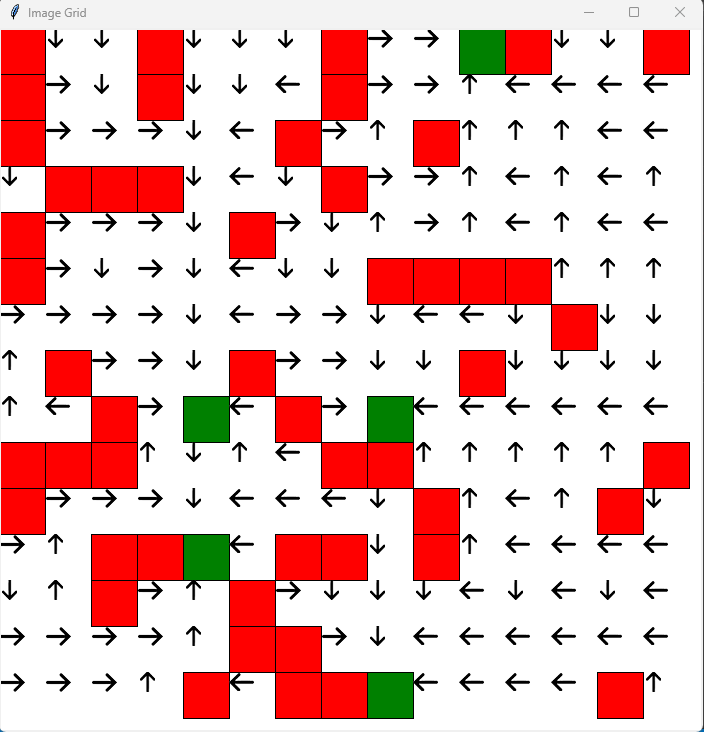
\includegraphics[width=0.5\textwidth, height=0.3\textheight]{grid_3.png}
  \caption{Third Run}
\end{figure}

\\~\\
\textbf{Note: Sometimes the algorithm gets trapped in opposite states selecting each other. If this happens the episode will get stuck. The algorithm needs to be run again in this case.}

\end{document}